Essa etapa consiste na implementação do DPD em FPGA. Para isso, é necessário realizar paralelizações nas operações aritméticas. A Figura \ref{fig:diagramaprocess} ilustra como esse processo está dividido entre cada ciclo de clock. A cada ciclo, duas operações são realizadas em paralelo: o sinal atual é elevado ao quadrado e registrado, enquanto ocorre o somatório do produto entre os sinais do mesmo instante de tempo e seus respectivos coeficientes. Esse processo ocorre P vezes para os \( P \) graus do polinômio de memória. Portanto, a saída do DPD é incompleta para os primeiros \( P \) períodos de clock, pois, nesses primeiros ciclos, realiza-se o cálculo com base em entradas de sinais anteriores que ainda não ocorreram, resultando em uma saída incompleta.

\begin{figure}[ht!]
	\centering
	\captionsetup{justification=centering}
	\caption*{Fonte: Autor}
	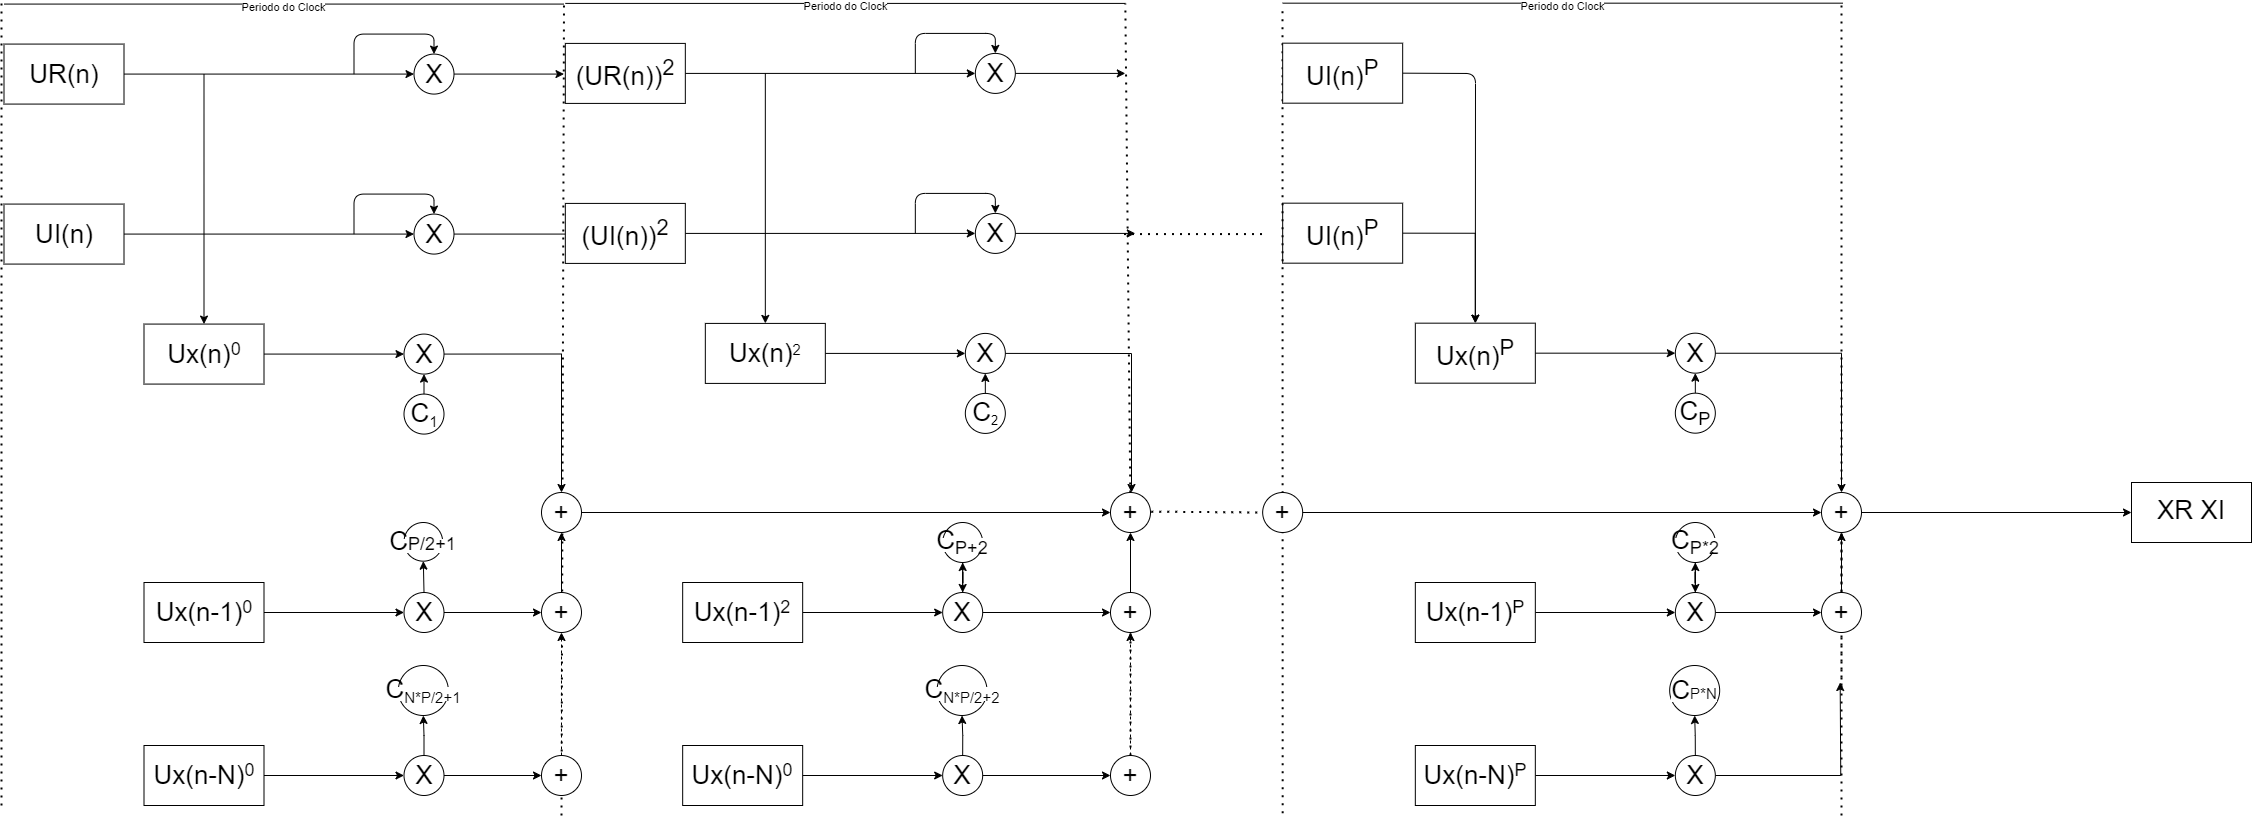
\includegraphics[width=1.0\textwidth]{diagrama_process.png}
	\caption{Processo de cálculo da saída}
	\label{fig:diagramaprocess}
\end{figure}